Drei Körper A, B und C bewegen sich auf geraden Bahnen. Die Stroboskopbilder zeigen ihre Orte im Abstand von $\tau = \dTO$, jeweils von links nach rechts.
\begin{center}
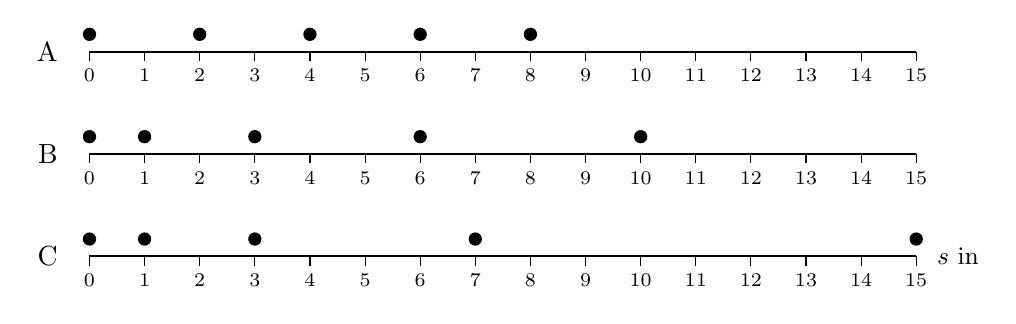
\begin{tikzpicture}[x=0.7cm, y=1cm]
 \draw[thick] (0,0) -- (15,0);
 \foreach \sk in {0,...,15} \draw (\sk,0) -- (\sk,-0.12);
 \foreach \sk in {0,1,...,15} \node[below, font=\scriptsize] at (\sk,-0.1) {$\sk$};
 \node[left] at (-0.4,0) {A};
 \fill[black] (0,0.22) circle (2.4pt);
 \fill[black] (2,0.22) circle (2.4pt);
 \fill[black] (4,0.22) circle (2.4pt);
 \fill[black] (6,0.22) circle (2.4pt);
 \fill[black] (8,0.22) circle (2.4pt);
 \draw[thick] (0,-1.3) -- (15,-1.3);
 \foreach \sk in {0,...,15} \draw (\sk,-1.3) -- (\sk,-1.42);
 \foreach \sk in {0,1,...,15} \node[below, font=\scriptsize] at (\sk,-1.4) {$\sk$};
 \node[left] at (-0.4,-1.3) {B};
 \fill[black] (0,-1.08) circle (2.4pt);
 \fill[black] (1,-1.08) circle (2.4pt);
 \fill[black] (3,-1.08) circle (2.4pt);
 \fill[black] (6,-1.08) circle (2.4pt);
 \fill[black] (10,-1.08) circle (2.4pt);
 \draw[thick] (0,-2.6) -- (15,-2.6);
 \foreach \sk in {0,...,15} \draw (\sk,-2.6) -- (\sk,-2.72);
 \foreach \sk in {0,1,...,15} \node[below, font=\scriptsize] at (\sk,-2.7) {$\sk$};
 \node[left] at (-0.4,-2.6) {C};
 \fill[black] (0,-2.38) circle (2.4pt);
 \fill[black] (1,-2.38) circle (2.4pt);
 \fill[black] (3,-2.38) circle (2.4pt);
 \fill[black] (7,-2.38) circle (2.4pt);
 \fill[black] (15,-2.38) circle (2.4pt);
 \node[right, font=\small] at (15.2,-2.6) {$s$ in \si{\meter}};
\end{tikzpicture}
\end{center}
Welche Bewegung ist gleichförmig, welche gleichmässig beschleunigt, welche keins von beiden? \DuSie{Bestimme}{Bestimmen Sie} die Geschwindigkeit der gleichförmigen und die Beschleunigung der gleichmässig beschleunigten Bewegung.
